\chapter{Symmetrische Kryptographie}

Bei symmetrischer Kryptographie verwenden Sender und Empfänger denselben Schlüssel, das heißt die Ver- und Entschlüsselung passieren symmetrisch.
Bei Verschlüsselung gibt es zwei Arten:

\paragraph{Blockcipher}\index{Blockcipher} Die Daten werden in Blöcke fixer Größe aufgeteilt und verschlüsselt. Das ist sinnvoll, wenn es keine zeitliche Komponente bei 
den Daten gibt, 
und sie zum Zeitpunkt der Verschlüsselung bereits vollständig vorhanden sind. 

\paragraph{Streamcipher}\index{Streamcipher} Die Daten werden verschlüsselt, sobald sie zu Verfügung stehen, und werden dann laufend mit dem 
Schlüsselstrom\index{Schlüsselstrom}\index{Keystream} verknüpt. 
Das erfordert Synchronisation zwischen Sender und Empfänger. Dieser Verschlüsselungsmodus ist für zeitkritische Anwendungen geeignet, bei denen man nicht warten kann, bis 
ein kompletter Block an Daten vorhanden ist.

Bei beiden Varianten ist die wichtigste Voraussetzung, den verwendeten Schlüssel sicher zu übertragen.

\section{Blockcipher}

\begin{definition}[Blockcipher]\index{Blockcipher}
Ein Blockcipher mit einer Blocklänge von $n$ Bit ist eine invertierbare, üblicherweise deterministische Abbildung.

Sei $V_n = \{0, 1\}^n$ die Menge aller $n$ Bit Vektoren und $\mathcal{K} = \{0, 1\}^k$ die Menge aller $k$ Bit Vektoren, dann sind

$$E: V_n \times \mathcal{K} \to V_n \text{ und } D: V_n \times \mathcal{K} \to V_n$$

mit $E(m, \kappa) = c$ für ein beliebiges $m \in V_n, \kappa \in \mathcal{K}$ und $D(c, \kappa) = m$ ein Blockcipher.
\end{definition}

Wir verwenden die Notation $E_K(p) = E(p, K)$ für die Verschlüsselung mit dem fixen Schlüssel $K \in \mathcal{K}$ und analog $D_K(C)$ für die Entschlüsselung. Dann gilt 
für alle $P \in V_n$, dass $D_K(E_K(P)) = P$.

Die Sicherheit, aber auch die Komplexität wird durch die Blocklänge beeinflusst, hier muss ein Tradeoff gemacht werden. Es gilt es die Blocklänge unter Berücksichtigung 
der sicherheitstechnischen und performanten Anforderungen zu wählen. \\

Die Auswahlkriterien für Blockcipher sind:

\begin{itemize}
    \item Geschätztes Sicherheitslevel: Je bekannter und erforschter ein Cipher ist, als desto sicherer wird er angesehen
    \item Schlüsselgröße: Je höher die Entropie der Schlüsselt, desto höher ist die Sicherheit. Mit der Entropie steigt aber auch der Verarbeitungsaufwand.
    \item Durchsatz: Der Durchsatz eines Ciphers ist abhängig von seiner Komplexität.
    \item Blockgröße: Je größer die Blockgröße, desto höher die Sicherheit, aber auch die Komplexität.
    \item Komplexität der kryptographischen Abbildung: Sie beeinflusst die Größe sowohl einer Software- als auch einer Hardwareimplementierung.
    \item Datenexpansion: Gewisse Anwendungen erfordern, dass Daten vor und nach der Verschlüsselung dieselbe Größe haben.
    \item Fehlerfortpflanzung: Ein fehlerhafter Ciphertext hat Auswirkungen auf Klartext, die konkrete Auswirkung unterscheidet sich je nach Betriebsmodus und Cipher.
\end{itemize}

\subsection{ECB (Electronic Codebook Mode)}\index{Blockcipher Modi!ECB}\index{ECB}

Die Verschlüsselung von Plaintext Block $p_i$ ist

\begin{align*}
    c_i = E_K(p_i) \\
    p_i = D_K(c_i)
\end{align*}

Die Vorteile des ECB sind: 

\begin{itemize}
    \item Wahlfreier Zugriff
    \item Fehler in Ciphertext beeinflusst nur aktuellen Block
    \item Wenn nur Nachrichten von bis zu einem Block übertragen werden, sicher und effizient
\end{itemize}

Die Nachteile sind:

\begin{itemize}
    \item Muster in Klartext im Ciphertext sichtbar
    \item Selber Klartext ergibt bei selbem Schlüssel immer selben Ciphertext
    \item Block Replay Attacken\index{Angriffe!Block Replay Attack}: beliebige Ciphertextblöcke können entfernt, eingefügt oder ersetzt werden
\end{itemize}


\subsection{CBC (Cipher Block Chaining)}\index{Blockcipher Modi!CBC}\index{CBC}

Die Verschlüsselung von Plaintext Block $p_i$ ist

\begin{align*}
    c_i = E_K(p_i \oplus c_{i-1}) \\
    p_i = c_{i-1} \oplus D_K(c_i)
\end{align*}

Die Vorteile des CBC sind: 

\begin{itemize}
    \item Gleiche Klartextblöcke ergeben nur dann gleiche Ciphertextblöcke, wenn vorhergehende Klartextblöcke identisch sind
    \item Kein Block Replay mehr möglich
    \item Auf Block Ebene selbstheilend
\end{itemize}

Die Nachteile sind:

\begin{itemize}
    \item Ent- und Verschlüsselung können nicht mehr wahlfrei erfolgen
    \item Vor allem am Beginn oft gleiche Klartextblöcke, Lösung: zufälliger IV, braucht nicht geheim gehalten zu werden
    \item Ein 1-Bit Fehler in Cipherblock $c_i$ bewirkt einen völlig fehlerhaften Klartextblock $p_i$ und einen 1-Bit Fehler in $p_{i+1}$ (``Error Extension'')
    \item Einfügen beliebiger Blöcke am Ende bzw. gezielte Manipulation von Block $p_{i+1}$ möglich
\end{itemize}

\subsection{PCBC (Propagating Cipher Block Chaining)}\index{Blockcipher Modi!PCBC}\index{PCBC}

Die Verschlüsselung von Plaintext Block $p_i$ ist

\begin{align*}
    c_i = E_K(p_i \oplus c_{i-1} \oplus p_{i-1}) \\
    p_i = c_{i-1} \oplus p_{i-1} \oplus D_K(c_i)
\end{align*}

Die Vorteile des PCBC sind: 

\begin{itemize}
    \item Grundsätzlich gleiche Eigenschaften wie CBC
    \item Zusätzlich: Fehler im Ciphertext bewirkt Fehler in allen folgenden Blöcken
    \item Verwendet in Kerberos 4 zum Error-checking: wenn der letzte Block nicht dem erwarteten Wert entspricht, ist ein Fehler aufgetreten.
\end{itemize}

Die Nachteile sind:

\begin{itemize}
    \item Grundsätzlich gleiche Eigenschaften wie CBC
    \item Vertauschen zweier Ciphertext Blöcke führt zu teilweiser falscher Entschlüsselung, wegen XOR fällt Fehler aber beim nächsten Block wieder heraus
\end{itemize}

\paragraph{Beispiel} Vertauschen zweier Blöcke:

Wir berechnen den Ciphertext von der Nachricht $P = (P_1, P_2, P_3, P_4, P_5)$ und Initialisierungsvektor $IV$:

\begin{align*}
    C_1 &= E_K(P_1 \oplus IV) \\
    C_2 &= E_K(P_2 \oplus C_1 \oplus P_1) \\
    C_3 &= E_K(P_3 \oplus C_2 \oplus P_2) \\
    C_4 &= E_K(P_4 \oplus C_3 \oplus P_3) \\
    C_5 &= E_K(P_5 \oplus C_4 \oplus P_4) \\
\end{align*}

Und erhalten $C = (IV, C_1, C_2, C_3, C_4, C_5)$. Jetzt manipuliert ein Angreifer den Ciphertext und wir entschlüsseln statt $C$ den Text 
$C'= (IV, C_1, C_\mathbf{3}, C_\mathbf{2}, C_4, C_5)$. Wir entschlüsseln:

\begin{align*}
    P_1 &= D_K(C_1) \oplus IV = (P_1 \oplus IV) \oplus IV = P_1 \\
    P'_2 &= D_K(C_3) \oplus P_1 \oplus C_1 = (P_3 \oplus C_2 \oplus P_2) \oplus P_1 \oplus C_1 \\
    P'_3 &= D_K(C_2) \oplus P'_2 \oplus C_3 = (P_2 \oplus C_1 \oplus P_1) \oplus P'_2 \oplus C_3 \\
         &= (P_2 \oplus C_1 \oplus P_1) \oplus (P_3 \oplus C_2 \oplus P_2 \oplus P_1 \oplus C_1) \oplus C_3 = P_3 \oplus C_2 \oplus C_3\\
    P_4 &= D_K(C_4) \oplus P'_3 \oplus C_2 = (P_4 \oplus C_3 \oplus P_3) \oplus (P_3 \oplus C_2 \oplus C_3) \oplus C_2 = P_4\\
    P_5 &= D_K(C_5) \oplus P_4 \oplus C_4 = (P_5 \oplus C_4 \oplus P_4) \oplus P_4 \oplus C_4 = P_5
\end{align*}

Das heißt, aus dem Cipher $C' = (IV, C_1, C_3, C_2, C_4, C_5)$ ist der Plaintext 
$P' = (P_1, P_3 \oplus C_2 \oplus P_2 \oplus P_1 \oplus C_1,  P_3 \oplus C_2 \oplus C_3, P_4, P_5)$ entstanden und nur die vertauschten Blöcke sind fehlerhaft.

\subsection{XTS (oder XEX-TCB-CTS)}\index{Blockcipher Modi!XTS}\index{XTS}\index{XEX-TCB-CTS}

Für das Xor-Encrypt-Xor-based Tweaked CodeBook Mode with Cipher Text Stealing\index{Cipher Text Stealing} brauchen wir einen geteilten Schlüssel $K = K_1 || K_2$, ein Tweak $i$ mit einem dazugehörigen 
$j$ (z.B. ist $i$ die Blocknummer auf der Harddisk unf $j$ der entsprechende Sektor) und ein $\alpha$, das ein primitives Element in $GF(2^{128})$ ist. 
Es gilt für die Ver- und Entschlüsselung:

\begin{align*}
    c_j &= E_{K_1}\left(p_i \oplus (E_{K_2}(j) \oplus \alpha^i)\right) \oplus \left(E_{K_2}(j) \oplus \alpha^i\right) \\
    p_j &= D_{K_1}\left(c_i \oplus (E_{K_2}(j) \oplus \alpha^i)\right) \oplus \left(E_{K_2}(j) \oplus \alpha^i\right)
\end{align*}

\begin{figure}[h]
    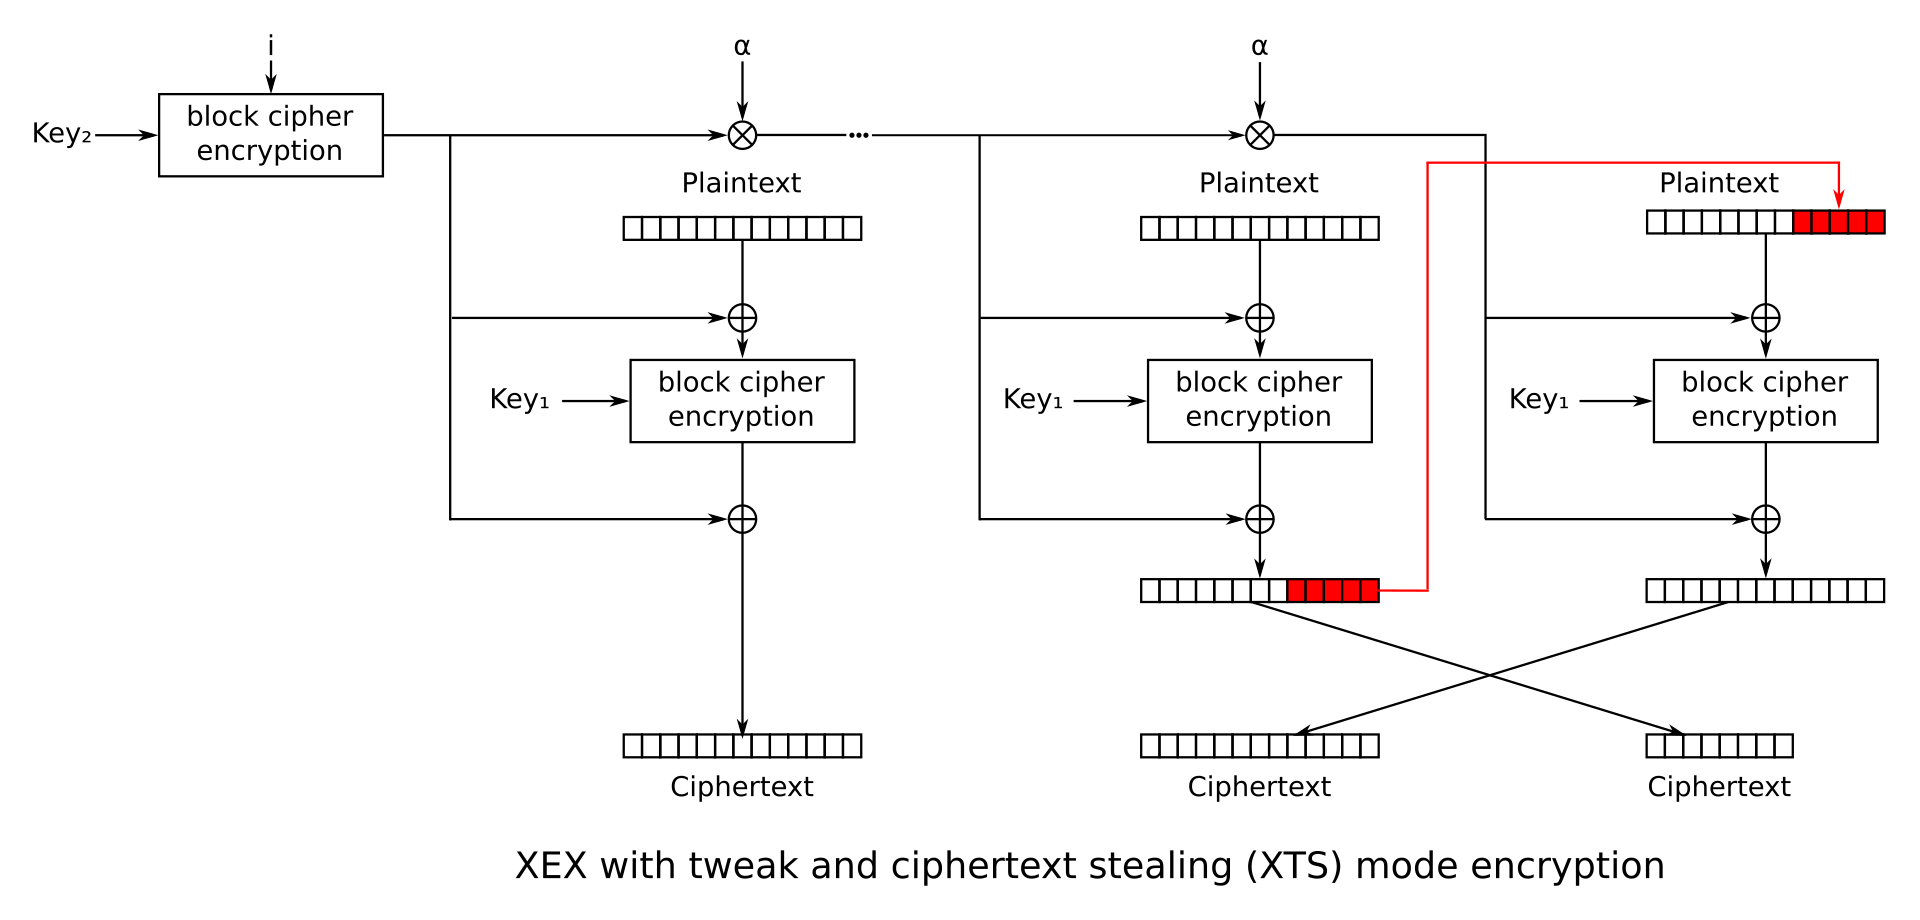
\includegraphics[width=0.8\textwidth]{figures/fig02-XTS_mode_encryption}
    \centering
    \caption{Aorimn, \href{https://creativecommons.org/licenses/by-sa/4.0}{CC BY-SA 4.0}, via Wikimedia Commons}
\end{figure}

Die Vorteile sind 

\begin{itemize}
    \item deal für Datenverschlüsselung an Endpunkten (Festplattenverschlüsselung)
    \item Ciphertext ist gleich lang wie Klartext
\end{itemize}

Die Nachteile sind

\begin{itemize}
    \item Schlüsselteilung ($K_1$ und $K_2$) potentiell unnötig und verkompliziert Vorgang
    \item Kein Authentication Tag
\end{itemize}

\subsection{Exkurs: CTS (Cipher Text Stealing)}\index{CTS}\index{Cipher Text Stealing}

Grundproblem: wenn der letzte Klartextblock kleiner ist als die Blockgröße, muss dieser aufgefüllt werden. Damit wird aber der Ciphertext größer als der Klartext. \\

Lösung: Sei $b$ die Blockgröße und $P = (P_1, \ldots, P_n)$ der Klartext.

\begin{enumerate}
    \item der letzte komplette Klartextblock $P_{-1}$ wird zu (Achtung) $C_\mathbf{n}$ verschlüsselt 
    \item der letzte Klartextblock $P_n$ wird mit den letzten $l$ Bits von $C_n$ aufgefüllt
    \item der neue letzter Block wird verschlüsselt, ergibt $C_\mathbf{n-1}$
    \item Die ersten $b-l$ Bits von $C_n$ ergeben den neuen letzten Block
\end{enumerate}

% width=0.8\textwidth
\begin{figure}[h]
    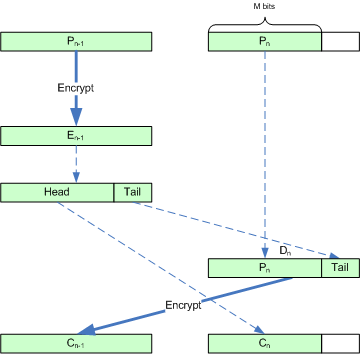
\includegraphics[width=0.4\textwidth]{figures/fig03-CTS_ECB_Encryption}
    \centering
    \caption{Yaronf, \href{https://creativecommons.org/licenses/by-sa/4.0}{CC BY-SA 4.0}, via Wikimedia Commons}
\end{figure}

\subsection{Auswahl des Blockcipher Modus}\index{Blockcipher Modi}

Folgende Empfehlungen gibt es für die Auswahl der Blockcipher Modi:

\begin{center}
    \begin{tabular}{ ll } 
        \hline
        Anwendungsfall & Modus \\ 
        \hline
        Kurze, zufällige Daten & (ECB) GCM \\
        Daten in der Übertragung & GCM \\
        Gespeicherte, große Daten & XTS \\
        \hline
    \end{tabular}
\end{center}

Andere Modi sind, wenn möglich, zu vermeiden.

\subsection{DES (Data Encryption Standard)}\index{DES}

Das NBS, der Vorläufer des heutigen NIST, beschloss 1972 einen standardisierten Verschlüsselungsalgorithmus zu entwickeln. Die Anforderungen daran waren:

\begin{itemize}
    \item Hohes Sicherheitslevel
    \item Leicht zu verstehen und lückenlos spezifiziert
    \item Sicherheit liegt im Schlüssel, nicht im Algorithmus
    \item Mit vertretbarem wirtschaftlichen Aufwand in elektronische Geräte integrierbar
    \item ``Frei'' verfügbar
    \item Anpassbar
    \item Effizient
    \item Validierbar
    \item Exportierbar
\end{itemize}

Beim ersten Aufruf gab es keine (brauchbaren) Einsendungen, beim zweiten (1974) dann eine von IBM, Lucifer. Dieser wurde mit Hilfe der NSA evaluiert, verändert und 
1975 veröffentlicht, ab 1976 Standard. DES wurde weitflächig übernommen, auch von Banken, Einzelhandel, Telekommunikation, etc.

Laut heutiger Aussage war die Veröffentlichung der ``größter Fehler der NSA'' - sie war der Meinung, es ginge bei DES nur um Hardwareimplementierungen.
Bis 1994 nur Hardware zertifiziert, keine Software. Ab 1983 wurde der Standard alle 5 Jahre reviewt:

\begin{itemize}
    \item 1983 problemlos
    \item 1988 Einspruch der NSA, ``likely to be broken''
    \begin{itemize}
        \item Als Alternative COMSEC
        \item Große Gegenwehr, Vorschlag abgelehnt
        \item NSA stimmte dann doch Rezertifizierung zu, mit Bedingung ``nie wieder''
    \end{itemize}
    \item 1993 wieder zertifiziert
    \item 1999 ebenso, mit Empfehlung, 3DES zu verwenden
    \item 2004 Standard (FIPS 46-3) zurückgezogen
\end{itemize}

DES ist ein symmetrischer Blockcipher mit Blockgröße 64 Bit. Die Schlüsselgröße ist 64 Bit, aber effektiv nur 56, da jedes 8.Bit ein Prüfbit ist. \\

Die Grundprinzipien ist Konfusion und Diffusion: Konfusion \index{Konfusion}\index{Blockcipher!Konfusion} heißt, die Beziehung zwischen Klartext, Schlüssel und Ciphertext soll so komplex wie möglich 
sein.
Diffusion \index{Diffusion}\index{Blockcipher!Diffusion} heißt, der Ciphertext hängt von so vielen Klartext Bits ab wie nur möglich.

DES wird mittels Permutationen und Substitutionen realisiert, die 16 Mal (als ``Runden'') wiederholt werden. Diese Struktur eignet sich sehr gut für 
Hardwareimplementierungen.

\begin{enumerate}
    \item Der 64-Bit Input wird initial permutiert.
    \item Das Ergebnis vom letzten Schritt wird in zwei Hälften $L_0$ und $R_0$ gespalten
    \item In einer Schleife wird 16 Mal ein Folgeergebnis berechnet: 
    \begin{enumerate}
        \item $L_i = R_{i-1}$
        \item $R_i = L_{i-1} \oplus f(R_{i-1}, K_i)$
    \end{enumerate}
    \item Für das Endergebnis werden beide Hälften zusammengefügt und final permutiert, das Ergebnis hat wie der Input 64 Bit.
\end{enumerate}

Die Entschlüsselung erfolgt bei DES völlig symmetrisch zur Verschlüsselung, einzig die Rundenkeys müssen in umgekehrter Reihenfolge erzeugt und verwendet werden.

Die zertifizierten Modi von DES sind ECB, CBC, OFB (Output Feedback Mode) und CFB (Cipher feedback). Implementierungen: zwischen 700 Mbit/sec (Software, OpenSSL) und 
768.000.000.000 keys/sec (Hardware, crack.sh). Der DES wird heute nicht mehr weiterentwickelt.

Betrachten wir die einzelnen Schritte:

\paragraph{Initiale und finale Permutation}

Die finale Permutation ist invers zur initialen.
Diese Permutation haben keinen Einfluss auf die Sicherheit, sondern wurden eingeführt um das Einlesen der Bytes in Hardware zu erleichtern. Bei Softwareimplementierungen 
werden sie oft ausgelassen, weil sie dort schwer und mit vielen Bitoperationen implementiert werden müssten.

\begin{figure}[h]
    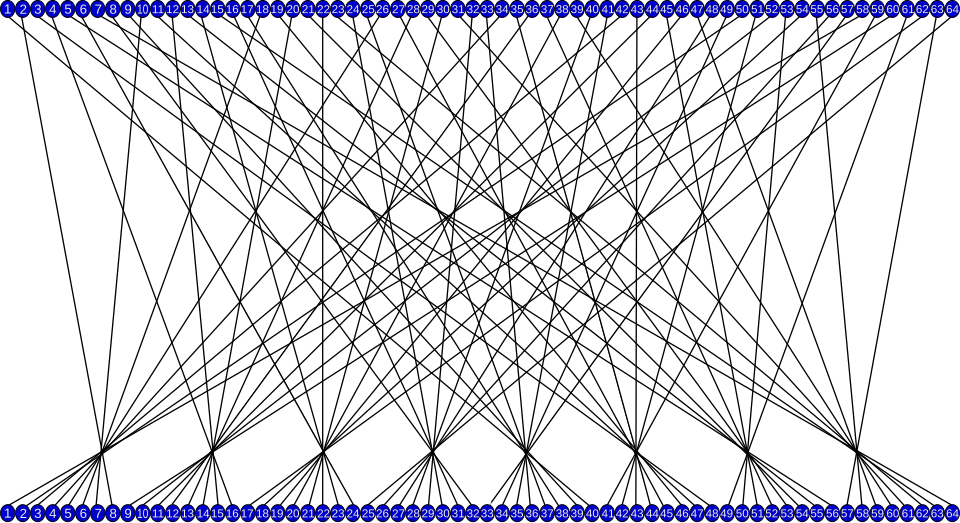
\includegraphics[width=0.8\textwidth]{figures/fig04-Permutation_initiale.png}
    \centering
    \caption{Initiale Permutation der 64 Bit, Quelle: Bourrichon, \href{https://creativecommons.org/licenses/by-sa/4.0}{CC BY-SA 4.0}, via Wikimedia Commons}
\end{figure}

\paragraph{Key Transformation mit Compression Permutation}

Bei der Key Transformation wird vom 64-Bit Key jedes 8. Bit verworfen. Die übrigen Bits werden in zwei Hälften zu je 28 Bit geteilt und in 16 Runden zirkulär nach links 
geshiftet. Dabei wird fast immer um 2 Bit geshiftet, außer in Runden 1, 2, 9 und 16, wo nur um 1 Bit geshiftet wird.

\begin{table}[h]
    \centering
        \begin{tabular}{|*{16}{c|}}
        \hline
        % Row 1 (cells 1-16)
        \cellcolor{red-1}1 & \cellcolor{red-1}2 & \cellcolor{red-1}3 & \cellcolor{red-1}4 & 
        \cellcolor{red-1}5 & \cellcolor{red-1}6 & \cellcolor{red-1}7 & \cellcolor{red-1}8 & 
        \cellcolor{yellow-1}9 & \cellcolor{yellow-1}10 & \cellcolor{yellow-1}11 & \cellcolor{yellow-1}12 & 
        \cellcolor{yellow-1}13 & \cellcolor{yellow-1}14 & \cellcolor{yellow-1}15 & \cellcolor{yellow-1}16 \\
        \hline
        % Row 2 (cells 17-32)
        \cellcolor{green-1}17 & \cellcolor{green-1}18 & \cellcolor{green-1}19 & \cellcolor{green-1}20 & 
        \cellcolor{green-1}21 & \cellcolor{green-1}22 & \cellcolor{green-1}23 & \cellcolor{green-1}24 & 
        \cellcolor{blue-1}25 & \cellcolor{blue-1}26 & \cellcolor{blue-1}27 & \cellcolor{blue-1}28 & 
        \cellcolor{blue-1}29 & \cellcolor{blue-1}30 & \cellcolor{blue-1}31 & \cellcolor{blue-1}32 \\
        \hline
        % Row 3 (cells 33-48)
        \cellcolor{orange-1}33 & \cellcolor{orange-1}34 & \cellcolor{orange-1}35 & \cellcolor{orange-1}36 & 
        \cellcolor{orange-1}37 & \cellcolor{orange-1}38 & \cellcolor{orange-1}39 & \cellcolor{orange-1}40 & 
        \cellcolor{purple-1}41 & \cellcolor{purple-1}42 & \cellcolor{purple-1}43 & \cellcolor{purple-1}44 & 
        \cellcolor{purple-1}45 & \cellcolor{purple-1}46 & \cellcolor{purple-1}47 & \cellcolor{purple-1}48 \\
        \hline
        % Row 4 (cells 49-64)
        \cellcolor{cyan-1}49 & \cellcolor{cyan-1}50 & \cellcolor{cyan-1}51 & \cellcolor{cyan-1}52 & 
        \cellcolor{cyan-1}53 & \cellcolor{cyan-1}54 & \cellcolor{cyan-1}55 & \cellcolor{cyan-1}56 & 
        \cellcolor{magenta-1}57 & \cellcolor{magenta-1}58 & \cellcolor{magenta-1}59 & \cellcolor{magenta-1}60 & 
        \cellcolor{magenta-1}61 & \cellcolor{magenta-1}62 & \cellcolor{magenta-1}63 & \cellcolor{magenta-1}64 \\
        \hline
        \end{tabular}
    \caption{Input Array für den Schlüssel mit 64 Bit}
\end{table}

\begin{table}[h]
    \centering
    \begin{minipage}[t]{0.45\textwidth}
        \begin{tabular}{|*{7}{c|}}
            \hline
            \cellcolor{magenta-1}57 & \cellcolor{cyan-1}49 & \cellcolor{purple-1}41 & \cellcolor{orange-1}33 & 
            \cellcolor{blue-1}25 & \cellcolor{green-1}17 & \cellcolor{yellow-1}9 \\

            \hline
            \cellcolor{red-1}1 & \cellcolor{magenta-1}58 & \cellcolor{cyan-1}50 & \cellcolor{purple-1}42 & 
            \cellcolor{orange-1}34 & \cellcolor{blue-1}26 & \cellcolor{green-1}18 \\

            \hline
            \cellcolor{yellow-1}10 & \cellcolor{red-1}2 & \cellcolor{magenta-1}59 & \cellcolor{cyan-1}51 & 
            \cellcolor{purple-1}43 & \cellcolor{orange-1}35 & \cellcolor{blue-1}27 \\

            \hline
            \cellcolor{green-1}19 & \cellcolor{yellow-1}11 & \cellcolor{red-1}3 & \cellcolor{magenta-1}60 & 
            \cellcolor{cyan-1}52 & \cellcolor{purple-1}44 & \cellcolor{orange-1}36  \\
            \hline
        \end{tabular}
    \end{minipage}
    \hfill
    \begin{minipage}[t]{0.45\textwidth}
        \begin{tabular}{|*{7}{c|}}
            \hline
            \cellcolor{magenta-1}63 & \cellcolor{cyan-1}55 & \cellcolor{purple-1}47 & \cellcolor{orange-1}39 & 
            \cellcolor{blue-1}31 & \cellcolor{green-1}23 & \cellcolor{yellow-1}15 \\

            \hline
            \cellcolor{red-1}7 & \cellcolor{magenta-1}62 & \cellcolor{cyan-1}54 & \cellcolor{purple-1}46 & 
            \cellcolor{orange-1}38 & \cellcolor{blue-1}30 & \cellcolor{green-1}22 \\

            \hline
            \cellcolor{yellow-1}14 & \cellcolor{red-1}6 & \cellcolor{magenta-1}61 & \cellcolor{cyan-1}53 & 
            \cellcolor{purple-1}45 & \cellcolor{orange-1}37 & \cellcolor{blue-1}29 \\

            \hline
            \cellcolor{green-1}21 & \cellcolor{yellow-1}13 & \cellcolor{red-1}5 & \cellcolor{blue-1}28 & 
            \cellcolor{green-1}20 & \cellcolor{yellow-1}12 & \cellcolor{red-1}4  \\
            \hline
        \end{tabular}
    \end{minipage}
    \caption{Output Arrays mit den Schlüsseln $K_1$ und $K_2$}
\end{table}

Nach dem Shiften werden aus den übrigen 56 Bits 48 ausgewählt und permutiert (``Compression Permutation''\index{Compression Permutation}):

\begin{table}[h]
    \centering
    \begin{tabular}{|*{14}{c|}}
        \hline
        % Row 1 
        \cellcolor{red-1}1 & \cellcolor{red-1}2 & \cellcolor{red-1}3 & \cellcolor{red-1}4 & 
        \cellcolor{red-1}5 & \cellcolor{red-1}6 & \cellcolor{red-1}7 & \cellcolor{red-1}8 & 
        \cellcolor{orange-1}9 & \cellcolor{orange-1}10 & \cellcolor{orange-1}11 & \cellcolor{orange-1}12 & 
        \cellcolor{orange-1}13 & \cellcolor{orange-1}14\\
        \hline
        % Row 2 
        \cellcolor{orange-1}15 & \cellcolor{orange-1}16 & 
        \cellcolor{yellow-1}17 & \cellcolor{yellow-1}18 & \cellcolor{yellow-1}19 & \cellcolor{yellow-1}20 & 
        \cellcolor{yellow-1}21 & \cellcolor{yellow-1}22 & \cellcolor{yellow-1}23 & \cellcolor{yellow-1}24 & 
        \cellcolor{green-1}25 & \cellcolor{green-1}26 & \cellcolor{green-1}27 & \cellcolor{green-1}28 \\
        \hline
        % Row 3 
        \cellcolor{green-1}29 & \cellcolor{green-1}30 & \cellcolor{green-1}31 & \cellcolor{green-1}32 &
        \cellcolor{cyan-1}33 & \cellcolor{cyan-1}34 & \cellcolor{cyan-1}35 & \cellcolor{cyan-1}36 & 
        \cellcolor{cyan-1}37 & \cellcolor{cyan-1}38 & \cellcolor{cyan-1}39 & \cellcolor{cyan-1}40 & 
        \cellcolor{blue-1}41 & \cellcolor{blue-1}42 \\
        \hline 
        % Row 4 
        \cellcolor{blue-1}43 & \cellcolor{blue-1}44 & 
        \cellcolor{blue-1}45 & \cellcolor{blue-1}46 & \cellcolor{blue-1}47 & \cellcolor{blue-1}48 &
        \cellcolor{purple-1}49 & \cellcolor{purple-1}50 & \cellcolor{purple-1}51 & \cellcolor{purple-1}52 & 
        \cellcolor{purple-1}53 & \cellcolor{purple-1}54 & \cellcolor{purple-1}55 & \cellcolor{purple-1}56 \\
        \hline
    \end{tabular}
    \caption{Input Array für mit 56 Bit}
\end{table}

\begin{table}[h]
    \centering
    \begin{tabular}{|*{12}{c|}}
        \hline
        % Row 1 
        \cellcolor{orange-1}14 & \cellcolor{yellow-1}17 & \cellcolor{orange-1}11 & \cellcolor{yellow-1}24 & 
        \cellcolor{red-1}1 & \cellcolor{red-1}5 & \cellcolor{red-1}3 & \cellcolor{green-1}28 &
        \cellcolor{orange-1}15 & \cellcolor{red-1}6 & \cellcolor{yellow-1}21 & \cellcolor{orange-1}10 \\
        \hline 
        
        % Row 2 
        \cellcolor{yellow-1}23 & \cellcolor{yellow-1}19 & \cellcolor{orange-1}12 & \cellcolor{red-1}4 & 
        \cellcolor{green-1}26 & \cellcolor{red-1}8 & \cellcolor{orange-1}16 & \cellcolor{red-1}7 & 
        \cellcolor{green-1}27 & \cellcolor{yellow-1}20 & \cellcolor{orange-1}13 & \cellcolor{red-1}2 \\
        \hline

        
        % Row 3  
        \cellcolor{blue-1}41 & \cellcolor{purple-1}52 & \cellcolor{green-1}31 & \cellcolor{cyan-1}37 & 
        \cellcolor{blue-1}47 & \cellcolor{purple-1}55 & \cellcolor{green-1}30 & \cellcolor{cyan-1}40 & 
        \cellcolor{purple-1}51 & \cellcolor{blue-1}45 & \cellcolor{cyan-1}33 & \cellcolor{blue-1}48 \\
        \hline

        % Row 4 
        \cellcolor{blue-1}44 & \cellcolor{purple-1}49 & \cellcolor{cyan-1}39 & \cellcolor{purple-1}56 &
        \cellcolor{cyan-1}34 & \cellcolor{purple-1}53 & \cellcolor{blue-1}46 & \cellcolor{blue-1}42 &
        \cellcolor{purple-1}50 & \cellcolor{cyan-1}36 & \cellcolor{green-1}29 & \cellcolor{green-1}32 \\
        \hline
    \end{tabular}
    \caption{Output Array nach ``Compression Permutation'' (48 bit)}
\end{table}

\begin{itemize}
    \item Weil jedes 8te Bit im Key ein Parity Bit ist, ist die faktische Länge des Keys statt 64 nur 56 Bit. 
    \item Für jede Runde muss ein anderer Schlüssel verwendet werden 
    \item Shiften ist schnell und billig in HW implementierbar 
    \item In keiner Runde wird der gesamte Schlüssel verwendet 
    \item Sicher gegen Related Key Analysis
\end{itemize}

\paragraph{Expansion Permutation}

In jeder Runde wird die Hälfte $R_i$ (32 Bit) mit dem 48 Bit Key xor-t werden. Dafür wird die Expansion Permutation \index{Expansion Permutation} verwendet. Hier gibt
es einen Lawinen Effekt (Avalanche Effect), wo möglichst viele Input Bits den Output beeinflussen (und umgekehrt). Das jeweils 1. und 4. Bit eines Blocks wird verdoppelt.

\begin{table}[h]
    \centering
    \begin{tabular}{|*{8}{c|}}
        \hline
        % Row 1 
        \cellcolor{red-1}1 & \cellcolor{red-1}2 & \cellcolor{red-1}3 & \cellcolor{red-1}4 & 
        \cellcolor{red-1}5 & \cellcolor{red-1}6 & \cellcolor{red-1}7 & \cellcolor{red-1}8 \\
        \hline 
        % Row 2 
        \cellcolor{orange-1}9 & \cellcolor{orange-1}10 & \cellcolor{orange-1}11 & \cellcolor{orange-1}12 & 
        \cellcolor{orange-1}13 & \cellcolor{orange-1}14 & \cellcolor{orange-1}15 & \cellcolor{orange-1}16 \\
        \hline 
        % Row 3
        \cellcolor{yellow-1}17 & \cellcolor{yellow-1}18 & \cellcolor{yellow-1}19 & \cellcolor{yellow-1}20 & 
        \cellcolor{yellow-1}21 & \cellcolor{yellow-1}22 & \cellcolor{yellow-1}23 & \cellcolor{yellow-1}24 \\
        \hline
        % Row 4 
        \cellcolor{green-1}25 & \cellcolor{green-1}26 & \cellcolor{green-1}27 & \cellcolor{green-1}28 &
        \cellcolor{green-1}29 & \cellcolor{green-1}30 & \cellcolor{green-1}31 & \cellcolor{green-1}32 \\
        \hline 
    \end{tabular}
    \caption{Input Array $R_i$ (32 Bit)}
\end{table}

\begin{table}[h]
    \centering
    \begin{tabular}{|*{12}{c|}}
        \hline
        % Row 1 
        \cellcolor{green-1}32 &
        \cellcolor{red-1}1 & \cellcolor{red-1}2 & \cellcolor{red-1}3 & \cellcolor{red-1}4 & 
        \cellcolor{red-1}5 & \cellcolor{red-1}6 & \cellcolor{red-1}7 & \cellcolor{red-1}8 & \cellcolor{orange-1}9\\
        \hline 
        % Row 2 
        \cellcolor{red-1}8 &
        \cellcolor{orange-1}9 & \cellcolor{orange-1}10 & \cellcolor{orange-1}11 & \cellcolor{orange-1}12 & 
        \cellcolor{orange-1}13 & \cellcolor{orange-1}14 & \cellcolor{orange-1}15 & \cellcolor{orange-1}16 & \cellcolor{yellow-1}17 \\
        \hline 
        % Row 3
        \cellcolor{orange-1}16 &
        \cellcolor{yellow-1}17 & \cellcolor{yellow-1}18 & \cellcolor{yellow-1}19 & \cellcolor{yellow-1}20 & 
        \cellcolor{yellow-1}21 & \cellcolor{yellow-1}22 & \cellcolor{yellow-1}23 & \cellcolor{yellow-1}24 & \cellcolor{green-1}25\\
        \hline
        % Row 4 
        \cellcolor{yellow-1}24 &
        \cellcolor{green-1}25 & \cellcolor{green-1}26 & \cellcolor{green-1}27 & \cellcolor{green-1}28 &
        \cellcolor{green-1}29 & \cellcolor{green-1}30 & \cellcolor{green-1}31 & \cellcolor{green-1}32 & \cellcolor{red-1}1\\
        \hline 
    \end{tabular}
    \caption{Zwischenergebnis Array für Expansion Permutation}
\end{table}

\begin{table}[h]
    \centering
    \begin{tabular}{|*{12}{c|}}
        \hline
        % Row 1 
        \cellcolor{orange-1}14 & \cellcolor{yellow-1}17 & \cellcolor{orange-1}11 & \cellcolor{yellow-1}24 & \cellcolor{red-1}1 & 
        \cellcolor{red-1}5 & \cellcolor{red-1}3 & \cellcolor{green-1}28 & \cellcolor{orange-1}15 & \cellcolor{red-1}6 & 
        \cellcolor{yellow-1}21 & \cellcolor{orange-1}10 \\
        \hline 
        % Row 2 
        \cellcolor{yellow-1}23 & \cellcolor{yellow-1}19 & \cellcolor{orange-1}12 & \cellcolor{red-1}4 & \cellcolor{green-1}26 & 
        \cellcolor{red-1}8 & \cellcolor{orange-1}16 & \cellcolor{red-1}7 & \cellcolor{green-1}27 & \cellcolor{yellow-1}20 & 
        \cellcolor{orange-1}13 & \cellcolor{red-1}2 \\
        \hline 
        % Row 3
        \cellcolor{blue-1}41 & \cellcolor{blue-1}52 & \cellcolor{green-1}31 & \cellcolor{blue-1}37 & \cellcolor{blue-1}47 & 
        \cellcolor{blue-1}55 & \cellcolor{green-1}30 & \cellcolor{blue-1}40 & \cellcolor{blue-1}51 & \cellcolor{blue-1}45 & 
        \cellcolor{blue-1}33 & \cellcolor{blue-1}48 \\
        \hline
        % Row 4 
        \cellcolor{blue-1}44 & \cellcolor{blue-1}49 & \cellcolor{blue-1}39 & \cellcolor{blue-1}56 & \cellcolor{blue-1}34 & 
        \cellcolor{blue-1}53 & \cellcolor{blue-1}46 & \cellcolor{blue-1}42 & \cellcolor{blue-1}50 & \cellcolor{blue-1}36 & 
        \cellcolor{green-1}29 & \cellcolor{green-1}32 \\
        \hline 
    \end{tabular}
    \caption{Output Array nach Expansion Permutation (sic)}
\end{table}

\begin{itemize}
    \item Der Datenblock muss auf Schlüsselgröße erweitert werden
    \item Durch Wiederholung einzelner Bits breitet sich Einfluss des Inputs aufden Output schneller aus (ein Inputbit beeinflusst 2 S-Box Lookups)
\end{itemize}

\paragraph{S-Boxen}

Der expandierte Block $R_i$ wird mit dem komprimierten Rundenschlüssel ver-xor-t. Der resultierende 48 Bit Block wird in 8 6er-Blöcke aufgeteilt. Jeder dieser 6 Bit 
Blöcke kommt in eine eigene S-Box.

Jede S-Box enthält 4 Zeilen zu je 16 Spalten und hat 4 Bit große Einträge.

\begin{itemize}
    \item Bits (1, 6) indizieren die Zeile (00, 01, 10, 11)
    \item Bits (2, 3, 4, 5) indizieren die Spalte (0000, 0001, \ldots, 1111)
    \item Beispiel: Der 6 Bit Input \verb|100111| wird auf den Eintrag in Zeile 4 (\verb|11|), Spalte 4 (\verb|0011|) gemapped
\end{itemize}

Aus den 48 (= $8 \cdot 6$) Bit Input wird über eine nicht-lineare Operation so ein 32 (= $8 \cdot 4$) Output generiert. Dieser Schritt ist besonders wichtig in DES.

Die Designkriterien für die S-Boxen (vgl. Don Coppersmith, The Data Encryption Standard (DES) and its strength against attacks) waren: 
\begin{itemize}
    \item Wegen HW und Technologie Beschränkungen (1974) waren nicht mehr als 6 Input- und 4 Output-Bits möglich 
    \item Kein Output Bit darf nahe einer linearen Funktion der Input Bits sein 
    \begin{itemize}
        \item Für jedes Output Bit und jeder Menge der 6 Input Bits ist das XOR dieser Inputs in ca. 50\% der Fälle gleich dem Output Bit
    \end{itemize}
    \item Jeder mögliche 4-Bit Output wird angenommen
    \item Wenn sich 2 Inputs um 1 Bit unterschieden, unterschiedet sich der Output um mindestens 2 Bit
    \item Wenn sich 2 Inputs nur in den beiden mittleren Bits unterscheiden, unterscheidet sich der Output in mindestens 2 Bit
    \item Wenn die ersten beiden Bits zweier Inputs anders, die letzten beiden gleich sind, dann ist der Output niemals ident
\end{itemize}

\paragraph{P-Boxen}

Nach der Substitution werden die 32 Bit noch einmal permutiert. Zum Abschluss werden die 32 Bit noch mit der linken Datenhälfte ver-xor-t. 
Danach werden $R_i$ und $L_i$ vertauscht. (todo: Tabelle einfügen)

Die Designkriterien der P-Boxen waren:

\begin{itemize}
    \item Die Output Bits von Runde $i$ (4 Bit) werden so verteilt, dass
    \begin{itemize}
        \item zwei der Bits in der Folgerunde zu den ``mittleren'' Bits einer S-Box werden. 
        \item zwei der Bits in der Folgerunde zu den ``Endbits'' werden. 
        \item sechs unterschiedliche S-Boxen dadurch beeinflusst werden.
    \end{itemize}
\end{itemize}

\paragraph{DES Runden}

\begin{figure}[h]
    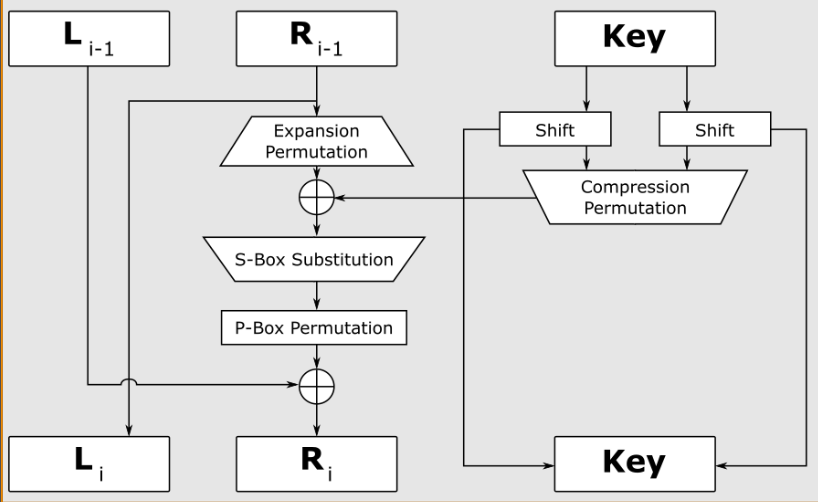
\includegraphics[width=0.8\textwidth]{figures/fig05-des-round.png}
    \centering
    \caption{Eine Runde in DES, Bruce Schneier, Applied Cryptography, 2nd Edition, Fig. 12.2}
\end{figure}


Nach 5 Runden ist jedes Outputbit eine Funktion jedes Input- und jedes Keybits.
Nach 8 Runden ist der Output quasi eine Zufallsfunktion -- aber durch differentielle Kryptoanalyse ((wieder)entdeckt 1990)
kann jede DES Implementierung innerhalb von 16 Runden gebrochen werden. 

\paragraph{Sicherheitsbetrachtungen div. Schlüssel}

Es gibt Weak Keys \index{Weak keys}, bei diesen besteht mindestens eine Hälfte (potentiell der gesamte Schlüssel) aus nur \verb|0| oder \verb|1|. Dadurch wird in jeder 
Runde derselbe Subkey erzeugt. Es gibt 4 verschiedene Weak Keys:

\begin{itemize}
    \item \verb|0x0101010101010101|
    \item \verb|0xFEFEFEFEFEFEFEFE|
    \item \verb|0xE0E0E0E0F1F1F1F1|
    \item \verb|0x1F1F1F1F0E0E0E0E|
\end{itemize}

Bei Semiweak Keys \index{Semiweak Keys} werden statt 16 unterschiedlicher Subkeys nur 2 erzeugt. Nachrichten die mit einem der Schlüsseln aus so einem Paar verschlüsselt 
werden, können auch mit dem anderen entschlüsselt werden. Von diesen Paaren gibt es 6:

\begin{itemize}
    \item \verb|0x011F011F010E010E| und \verb|0x1F011F010E010E01|
    \item \verb|0x01E001E001F101F1| und \verb|0xE001E001F101F101|
    \item \verb|0x01FE01FE01FE01FE| und \verb|0xFE01FE01FE01FE01|
    \item \verb|0x1FE01FE00EF10EF1| und \verb|0xE01FE01FF10EF10E|
    \item \verb|0x1FFE1FFE0EFE0EFE| und \verb|0xFE1FFE1FFE0EFE0E|
    \item \verb|0xE0FEE0FEF1FEF1FE| und \verb|0xFEE0FEE0FEF1FEF1|
\end{itemize}

Weiters gibt es auch Possibly Weak Keys, diese erzeugen nur 4 unterschiedliche Subkeys, von denen gibt es 48.\\

Die Eigenschaft Complement Keys \index{Complement Keys} beschreibt, dass das Einser-Komplement eines Schlüssels das Einser-Komplement eines Klartextes zum 
Einser-Komplement des Ciphertexts verschlüsselt: 

$$\text{DES}(p, k) = c \Rightarrow \text{DES}(\lnot p, \lnot k) = \lnot c$$

Damit muss ein Brute-Force Angreifer nur die Hälfte der Keys ausprobieren (trotzdem noch 255 Möglichkeiten).\\


Schlüssellänge: Der Erstvorschlag hatte 112 Bit Keys, die NSA wollte ihn auf 48 verkürzen, als Kompromiss hat man sich auf 56 Bit geeinigt.
Per Brute-Force konnte man 1977 $2^{56}$ Schlüssel schwer knacken, heute ist diese Aufgabe problemlos:

\begin{itemize}
    \item ``Deep Crack'', 1998, \$250.000, 56 Stunden
    \item COPACOBANA, 2006, \$10.000, unter 24 Stunden
    \item \url{www.cloudcracker.com}, 2013, \$20, 21 Stunden
    \item crack.sh, 2017, 26 Stunden
\end{itemize}

Variante zu Brute-Force: Klartextblock mit allen $2^{56}$ Schlüsseln verschlüsseln und speichern, dann in Übertragung diesen
Klartextblock einschleusen und Ciphertext abfangen. \\

Kryptoanalyse: 

\begin{itemize}
    \item Resistent gegen differentielle Krytanalyse, wenn alle 16 Runden verwendet
    \item Weniger resistent gegen lineare Kryptanalyse, aber immer noch $2^{43}$ Klartexte nötig
    \item Resistent gegen Related Key Kryptanalyse
\end{itemize}

Trotzdem: DES kann in seiner Urform heute nicht mehr als sicher angesehen werden!


\section{Strengthening}

\subsection{Mehrfache Verschlüsselung}

Grundidee: Klartext mit demselben Algorithmus, aber unterschiedlichen Schlüsseln, mehrmals verschlüsseln (denselben Schlüssel zu verwenden bringt keinerlei Gewinn).

\paragraph{Double Encryption}

Die Ver- und Entschlüsselung dieses Blockalgorithmus ist:

\begin{align*}
    c = E_{K_2}\left( E_{K_1}(p) \right) \\
    p = D_{K_1}\left( D_{K_2}(c) \right) \\
\end{align*}

Double Encryption ist nur sinnvoll, wenn der Blockalgorithmus keine algebraische Gruppe bildet (präziser: wenn er nicht abgeschlossen ist). Ansonsten gibt es immer ein 
$K_3$, sodass $c = E_{K_2}\left( E_{K_1}(p) \right) = E_{K_3}(p)$.

Eine naive Rechnung gibt uns die Erkenntnis, dass wir statt $2^n$ verschiedenen Schlüsseln nun $2^{2n}$ verschiedene Schlüssel haben.

Problem: Meet-in-the-Middle Attack\index{Angriffe!Meet-in-the-Middle Attack}\index{Meet-in-the-Middle Attack}, diese benötigt nur $2^{n+1}$ Versuche:

\begin{itemize}
    \item Ist eine Known-Plaintext Attacke 
    \item Der Angreifer kennt zwei Plaintext-Ciphertext Paare $(p_1, c_1)$ und $(p_2, c_2)$.
    \item Angreifer berechnet und speichert $E_K(p_1)$ für jeden möglichen Schlüssel $K$
    \item Danach berechnet er $D_K(c_1)$ für jedes $K$ und sucht diesen Wert unter den gespeicherten
    \item Wenn gefunden: aktuelles $K$ ist sehr wahrscheinlich $K_2$, und $K$ für Wert in Speicher war $K_1$, nachprüfbar mit $(p_2, c_2)$.
    \item Nicht praktikabel, aber weit besser als Brute-Force
    \begin{itemize}
        \item Meet-in-the-middle: $2\cdot 2^n = 2^{n+1}$ Verschlüsselungen, Speicheraufwand: $O(2^n)$
        \item Brute Force: $2^{2n}$ Verschlüsselungen, Speicheraufwand: $O(1)$
    \end{itemize}
\end{itemize}

\paragraph{Triple Encryption}

Die Ver- und Entschlüsselung dieses Blockalgorithmus ist ein Encryption-Decryption-Encryption Schema (EDE):

\begin{align*}
    c = E_{K_3}\left( D_{K_2} \left( E_{K_1}(p) \right) \right) \\
    p = D_{K_1}\left( E_{K_2} \left( D_{K_3}(c) \right) \right) \\
\end{align*}

In DES wird das als Triple-DES verwendet.

\begin{itemize}
    \item 3 Optionen:
    \begin{enumerate}
        \item $K_1 \neq K_2 \neq K_3$
        \item $K_1 = K_3$ und $K_1 \neq K_2$
        \item $K_1 = K_2 = K_3$
    \end{enumerate}
    \item Option 1 ergibt einen 168(=$3\cdot 56$)Bit Key (effektiv aber nicht stärker als 112 Bit)
    \item Option 2 ergibt 112-Bit Key, ist aber stärker als einfache Double Encryption (weil meet-in-the-middle jetzt einmal $K_1K_2$ raten muss)
    \item Option 3 ist effektiv wieder DES, existiert nur aus Abwärtskompatibilität (was auch der Grund für das EDE Muster ist, ansonsten wäre z.B. EEE genauso anwendbar)
    \item Beste Attacke ist wieder Variante von meet-in-the-middle\index{Meet-in-the-Middle Attack}\index{Angriffe!Meet-in-the-Middle Attack}, mit Komplexität $2^{2n}$ 
    (und damit der Komplexität, die man bei Double Encryption hätte erwarten 
    können)
    \item Triple-DES wird aktuell noch bis 2023 zur Verwendung erlaubt
    \item Auch andere Varianten möglich, z.B. Independent Subkeys, Key-dependent S-Boxes,\ldots
\end{itemize}

\subsection{Kaskadierung}

Bei Kaskadierung werden unterschiedliche Algorithmen hintereinander angewendet. Wenn die einzelnen Schlüssel unabhängig sind, ist die Kaskade mindestens so schwer zu 
brechen wie der erste Algorithmus in der Kaskade.

\subsection{Whitening}

Vor und nach der Verschlüsselung wird ein Teil des Schlüssels mit dem Input/Output verxort. Das verhindert, dass ein Angreifer Klartext/Geheimtext Paare bekommen kann.

\section{AES (Advanced Encryption Standard)}

Im Jänner 1997 wurde vom NIST ein Wettbewerb für einen DES Nachfolger ausgeschrieben.
AES ist seit Mai 2002 offizieller Standard. Der ursprünglicher Aufruf war ``an unclassified, publicly disclosed encryption algorithm capable of protecting sensitive 
government information well into the next century''.
Im September 1997 wurden die Anforderungen spezifiziert:

\begin{itemize}
    \item The algorithm must implement symmetric (secret) key cryptography.
    \item The algorithm must be a block cipher.
    \item The candidate algorithm shall be capable of supporting key-block combinations with sizes of 128-128, 192-128, and 256-128 bits. A submitted algorithm may support 
other key-block sizes and combinations, and such features will be taken into consideration during analysis and evaluation.
\end{itemize}

In der 1. Runde gab es 15 Einreichungen, von denen 5 in die nächste Runde kamen, nämlich 

\begin{itemize}
    \item MARS 
    \item RC6
    \item Rijndael 
    \item Serpent 
    \item Twofish
\end{itemize}

Der Sieger war Rijndael von Vincent \textbf{Rij}men und Joan \textbf{Dae}men. Bruce Schneier sagte 2000 über den Algorithmus 

\say{I believe that within the next five years someone will
discover an academic attack against Rijndael. I do not believe
that anyone will ever discover an attack that will allow
someone to read Rijndael traffic. So while I have serious
academic reservations about Rijndael, I do not have any
engineering reservations about Rijndael.}

\subsection{Exkurs: Arithmetik in $GF(2^m)$}

Wir betrachten die Arithmetik in binären Erweiterungskörpern.
Bezeichne $GF(2^m)$ die Menge aller binären Polynomen mit Grad $< m$.

\begin{itemize}
    \item Berechnungen modulo irreduziblem Polynom von Grad m
    \item m ist (z.B. bei elliptischen Kurven): (113), (131), 163, (176), 191, 193, 233, (239), (283), (409), 571
    \item Elemente dargestellt als Integer
    \begin{itemize}
        \item $x^3+x^2+1$ ist Element von $GF(2^4)$, dargestellt als $1101$
        \item für $GF(2^m)$ sind $m$ Bit notwendig
        \item Elemente aus $GF(2^8)$ passen exakt in ein Byte
    \end{itemize}
\end{itemize}

\paragraph{Operationen}

Sei $a(x) = x^3+x^2+x = 1110, b(x) = x^2+x+1 = 0111$ und $f(x) = x^4+x+1 = 10011$. Es gilt:

\begin{itemize}
    \item Addition/Subtraktion: Polynomaddition modulo 2, entspricht xor
        $$a + b = x^3+1 (1110 xor 0111 = 1001)$$
    \item Inversion bzgl. $f(x)$
        $$b^{-1} = x^2+x$$
    \item Multiplikation mod $f(x)$
        $$a \cdot b = x^5+x^3+x \mod f(x) = x^3+x^2$$
    \item Quadrierung mod $f(x)$ (einfache Spreizung)
    $$ a^2 = x^6+x^4+x^2 \mod f(x) (11102 = 1010100) = x^3+x+1$$
\end{itemize}

\paragraph{Übung}

Sei $a(x) = x^3 + x^2 + x, b(x) = x^2+x+1, c(x) = x^2+x$ und $f(x) = x^4+x+1$. Berechnen Sie

\begin{enumerate}
    \item $c + b$
    \item $a + b + c$
    \item $b - c$
    \item $c^2 \mod f$
    \item $b \cdot c \mod f$
    \item $c^{-1} \mod f$
\end{enumerate}

\subsection{Verschlüsselung}

Rijndael ist ein Blockcipher, die Block- und Schlüssellänge ist jedes Vielfache von 32 Bit zwischen inkl. 128 und inkl. 256 Bit.
Es verwendet kein Feistelnetzwerk, für jede Operation muss eine inverse Operation definiert werden.

Die Unterschiede zwischen Rijndael und AES sind:
\begin{itemize}
    \item AES Blocklänge ist immer 128 Bit
    \item AES Schlüssellängen
    \begin{itemize}
        \item 128 Bit (10 Runden)
        \item 192 Bit (12 Runden)
        \item 256 Bit (14 Runden)
    \end{itemize}
\end{itemize}

\begin{figure}[h]
    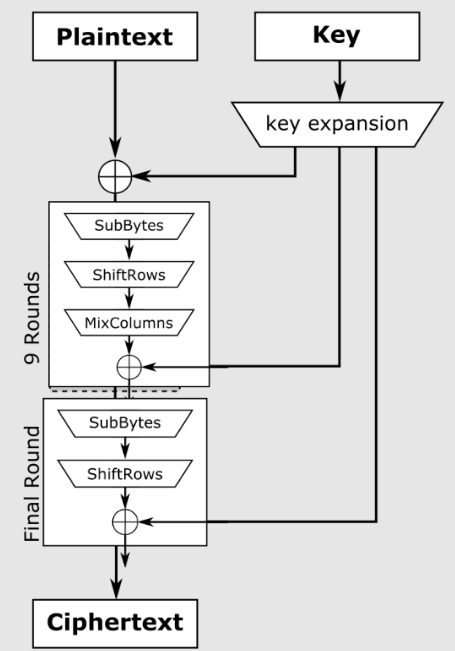
\includegraphics[width=0.5\textwidth]{figures/fig06-aes}
    \centering
    \caption{AES}
\end{figure}

Sei $b$ die Blocklänge des Ciphers. AES operiert auf einem State:
\begin{itemize}
    \item 2-dimensionales Bytearray mit 4 Zeilen und $b/32$ Spalten
    \item Sowohl Klartext als auch Schlüssel werden zu Beginn auf je ein solches Array gemappt
    \item Beispiel: bei 128 Bit Blocklänge ergibt sich ein $4 \times 4$ Array
\end{itemize}

\paragraph{Sub-Bytes} ist die einzige nicht-lineare Operation in AES. (? Todo: \verb|folien AK_02_block_v02.pdf|, Seite 65)

\begin{itemize}
    \item Konfusion
    \item S-Box 
    \item Die einzelnen Bytes werden als Elemente von $GF(2^8)$ betrachtet
    \item Irreduzibles Polynom ist $x^8 + x^4 + x^3 + x + 1$
    \item Jedes Byte $a_{i,j}$ wird transformiert zu $b_{i,j} = Sbox(a_{i, j}) = f(g(a_{i,j}))$ mittels 
    \begin{itemize}
        \item $g: a \mapsto a' = a^{-1}$
        \item $f: a' \mapsto b = A\cdot a' + v$
    \end{itemize}
    \item Affine Transformation mit $v$ um Attacken zu Vermeiden. 
\end{itemize}

\begin{equation*}
    A = \begin{pmatrix}
        1 & 1 & 1 & 1 & 1 & 0 & 0 & 0\\
        0 & 1 & 1 & 1 & 1 & 1 & 0 & 0\\
        0 & 0 & 1 & 1 & 1 & 1 & 1 & 0\\
        0 & 0 & 0 & 1 & 1 & 1 & 1 & 1\\
        1 & 0 & 0 & 0 & 1 & 1 & 1 & 1\\
        1 & 1 & 0 & 0 & 0 & 1 & 1 & 1\\
        1 & 1 & 1 & 0 & 0 & 0 & 1 & 1\\
        1 & 1 & 1 & 1 & 0 & 0 & 0 & 1\\
\end{pmatrix} \text{ und } v = (0,1,1,0,0,0,1,1)^\top
\end{equation*}

\paragraph{ShiftRows}

Diffusion:
\begin{itemize}
    \item Jede Zeile des States wird zyklisch nach links geshiftet
    \item Offsets: 0,1,2,3 für 128 Bit Blocklänge
    \item Mit diesen Offsets maximale Diffusion und größte Resistenz gegen bekannte Attacken
\end{itemize}

(todo: add graphic)

\paragraph{MixColumns}

Diffusion
\begin{itemize}
    \item Arbeitet auf den Spalten des States (wegen 32-Bit Architektur sind 4 Zeilen, d.h. 32 Bit pro Spalte optimal)
    \item Bytes einer Spalte werden Koeffizienten eines Polynoms vom Grad 3 in $GF(2^8)$ betrachtet
    \begin{itemize}
        \item Spalte wird multipliziert mit $03x^3 + 01x^2 + 01x + 02$
        \item Multiplikation mit 01 ist die Identität 
        \item Multiplikation mit 02 ist ein Shift und ein XOR 
        \item Multiplikation mit 03 ist eine Multiplikation mit 02 und ein XOR 
        \item Reduziert mit $x^4 + 1$ 
    \end{itemize}
\end{itemize}

De facto handelt es sich also um ein Polynom in $x$, dessen Koeffizienten Polynome sind. Herleitung daher allgemein einfacher.
Notation: statt $a_{i,j}$ steht im Folgenden $a_i$, zur Wahrung der Übersichtlichkeit. \\

Beispiel: Stelle 

\begin{align*}
    (02a_3+a_2+a_1+03a_0)&x^3 + \\
    (03a_3+02a_2+a_1+a_0)&x^2 + \\
    (a_3+03a_2+02a_1+a_0)&x^1 + \\ 
    (a_3+a_2+03a_1+02a_0)& 
\end{align*}
    
    als Matrix dar:

\begin{equation*}
    \begin{pmatrix}
        b_0 \\ b_1 \\ b_2 \\ b_3 \\
\end{pmatrix}  = \begin{pmatrix}
        02 & 03 & 01 & 01 \\
        01 & 02 & 03 & 01 \\
        01 & 01 & 02 & 03 \\
        03 & 01 & 01 & 02 \\
\end{pmatrix} \cdot \begin{pmatrix}
        a_0 \\ a_1 \\ a_2 \\ a_3 \\
\end{pmatrix} 
\end{equation*}

\paragraph{AddRoundKey}

Aktueller Rundenschlüssel wird byteweise mit aktuellem State verxort

\paragraph{Key Schedule}

Aus initialem 128-bit (bzw. 192 bzw. 256-bit) Key muss für jede
Runde ein Schlüssel in Blocklänge (128 Bit) generiert werden. Seo $b$ die Blocklänge und $r$ die Rundenanzahl.
Die zwei Schritte dafür sind:

\begin{enumerate}
    \item Key Expansion: wie wird aus initialem Schlüssel ein Schlüssel der Länge $(r + 1) \cdot b$ Bit
    \item Round Key Selection: wie wird Schlüsselteil für aktuelle Runde ausgewählt
\end{enumerate}


\begin{itemize}
    \item Schlüssel wird in 2-dimensionales Array geschrieben
    \item Die letzte Spalte des Arrays wird einmal zirkulär nach oben geshiftet
    \item Danach mittels S-Box aus SubBytes behandelt
    \item Dann mit Rundenkonstante verxort
    \begin{itemize}
        \item Runde 1: 0x01 (1, 01)
        \item Runde 2: 0x02 (x, 10)
        \item Runde 3: 0x04 (x2, 100)
        \item Runde 4: 0x08 (x3, 1000)
        \item Runde 5: 0x10 (x4, 1 0000)
        \item Runde 6: 0x20 (x5, 10 0000)
        \item Runde 7: 0x40 (x6, 100 0000)
        \item Runde 8: 0x80 (x7, 1000 0000)
        \item Runde 9: 0x1b (x8 mod (x8 + x4 + x3 + x + 1), 1 1011)
        \item Runde 10: 0x36 (x9 mod (x8 + x4 + x3 + x + 1), 11 0110)
    \end{itemize}
    \item Schließlich mit erster Spalte des letzten Rundenschlüssels verxort, ergibt erste Spalte des aktuellen Rundenschlüssels
    \item Übrige Spalten entstehen durch verxoren der vorherigen Spalte mit der entsprechenden Spalte des letzten Rundenschlüssels
(Spalte 2 des neuen Schlüssels ist also Spalte 1 des neuen verxort mit Spalte 2 des alten) 
\end{itemize}

\subsection{Entschlüsselung}

Für die Entschlüsselung brauchen wir für jede Funktion der Verschlüsselung ein Inverses:

\begin{center}
    \begin{tabular}{ ll } 
        \hline
        Verschlüsselung & Entschlüsselung \\ 
        \hline
        SubBytes & InvSubBytes \\
        ShiftRows & InvShiftRows \\
        MixColumns & InvMixColumns \\
        AddRoundKey & AddRoundKey (selbstinvers) \\
        \hline
    \end{tabular}
\end{center}

Weiters, muss die Reihenfolge der Operationen umgekehrt werden.
Möglichkeit einer mathematisch äquivalenten Beschreibung, um die Reihenfolge beizubehalten:

\begin{itemize}
    \item InvSubBytes und InvShiftRows können vertauscht werden, es ist völlig egal, ob Werte zuerst ersetzt und dann verschoben werden, oder umgekehrt
    \item InvMixColumns und AddRoundKey können vertauscht werden, weil InvMixColumns linear ist, d.h. $F(a\oplus b) = F(a) \oplus F(b)$
\end{itemize}

\noindent Damit ist wenn EquivRoundKey := InvMixColumns(RoundKey):

$$\text{InvMixColumns}(\text{State} \oplus \text{Roundkey}) = \text{InvMixColumns}(\text{State}) \oplus \text{EquivRoundKey}.$$ 

\paragraph{Beispiel} für 3 Runden:

\begin{center}
    \begin{tabular}{ lll } 
        \hline
        Verschlüsselung & $>$ Entschlüsselung & $>$ Entschlüsselung optimiert\\ 
        \hline
        AddRoundKey & AddRoundKey   & AddRoundKey \\
        SubBytes    & InvShiftRows  & InvSubBytes \\
        ShiftRows   & InvSubBytes   & InvShiftRows \\ 
        MixColumns  & AddRoundKey   & InvMixColumns \\
        AddRoundKey & InvMixColumns & EquivRoundKey \\
        SubBytes    & InvShiftRows  & InvSubBytes \\
        ShiftRows   & InvSubBytes   & InvShiftRows \\
        MixColumns  & AddRoundKey   & InvMixColumns \\
        AddRoundKey & InvMixColumns & EquivRoundKey \\
        SubBytes    & InvShiftRows  & InvSubBytes \\
        ShiftRows   & InvSubBytes   & InvShiftRows \\
        AddRoundKey & AddRoundKey   & AddRoundKey \\
        \hline
    \end{tabular}
\end{center}

\subsection{Zusammenfassung}

\paragraph{Effizienz}

\begin{itemize}
    \item Sämtliche Berechnungen können vorab als Lookup-Tables gespeichert werden
    \item SubBytes, ShiftRows und MixColumns können in einer Operation zusammengefasst werden
    \item Sowohl in Hardware als auch in Software schnell implementierbar
    \item Von 8-bit bis 128-bit Architekturen
    \item Intel mit eigenen Instruction Set Extensions für AES (z.B. \verb|AESENC|, \verb|AESENCLAST|, \verb|AESDEC|, \ldots)
\end{itemize}

\paragraph{Designentscheidungen}

\begin{itemize}
    \item Anzahl der Runden
    \begin{itemize}
        \item Volle Diffusion nach 2 Runden (mit Feistelnetzwerk nicht erreichbar)
        \item Änderung in einem State Bit beeinflusst ungefähr die Hälfte aller State Bits nach 2 Runden
        \item Keine Attacken für Versionen ab 6 Runden gefunden
        \item 4 Runden Security Margin hinzugefügt, damit also quasi je einmal volle Diffusion am Anfang und am Ende hinzugefügt
        \item Für je 32 Bit Schlüssellänge wird eine Runde hinzugefügt
        \item Für je 32 Bit Blocklänge wird eine Runde hinzugefügt (betrifft nur Rijndael)
    \end{itemize}
    \item SubBytes
    \begin{itemize}
        \item ist nicht-linear, erreicht durch Inversion in endlichem Körper
        \item Algebraisch Komplex, erreicht durch affine Transformation
    \end{itemize}
    \item ShiftRows
    \begin{itemize}
        \item Maximale Diffusion (4 unterschiedliche Offsets)
        \item Einfachste Variante bei mehreren gleichwertigen gewählt
    \end{itemize}
    \item MixColumns
    \begin{itemize}
        \item 4-Byte Spalten, um 32-Bit Architektur auszunützen
        \item Linear in $GF(2)$
        \item Diffusion, nicht zwangsläufig optimale
        \item Auch auf 8-Bit Architekturen gute Performance
    \end{itemize}
    \item KeyAddition und Key Schedule
    \begin{itemize}
        \item Durch Addition des Keys am Anfang und am Ende (siehe Whitening)
        \item Möglichst wenig Arbeitsspeicher für KeyExpansion durch rekursive Definition
        \item Symmetrien eliminiert durch Addition der Rundenkonstanten
        \item Diffusion
    \end{itemize}
\end{itemize}

\paragraph{Kritik und Angriffe}

Es gibt zwei große Kritikpunkte bzgl. AES: 

\begin{itemize}
    \item Einfachheit
    \begin{itemize}
        \item Großteil ist algebraisch zu beschreiben
        \item Ungewöhnlich für Blockcipher
    \end{itemize}
    \item Key Schedule 
    \begin{itemize}
        \item Attacken für 256 Bit Keys bekannt
    \end{itemize}
\end{itemize}

Die momentan besten Angriffe sind:

\begin{itemize}
    \item Auf AES-256, 14 Runden, in $O(2^{99.5})$
    \item Auf AES-192, 12 Runden, in $O(2^{176})$
    \item Auf AES-128, 10 Runden, in $O(2^{126.1})$
\end{itemize}


\section{Streamcipher}\index{Streamcipher}

Im Gegensatz zu Blockciphern werden hier Daten verschlüsselt, sobald sie zur
Verfügung stehen. Das wird überall dort gebraucht, wo Latenzen ein Problem bereiten.\\ 

\noindent Streamciphers sind üblicherweise sehr effizient in Hardware implementierbar. \\

\noindent Datenstrom wird mit einem Schlüsselstrom\index{Schlüsselstrom}\index{Keystream} verknüpft (üblicherweise per xor)m dafür muss der Schlüsselstrom gleich lang 
sein wie die Daten.
Im Idealfall ist der Schlüsselstrom eine komplette Zufallsfolge (siehe One-Time Pad). \\

\noindent Bei Streamciphern sind Konfusion und Diffusion nicht möglich. Das heißt die Sicherheit liegt allein in der Qualität des Schlüsselstroms. \\

\noindent Streamcipher werden sehr oft gerade in der Telekommunikationsbranche verwendet,
allerdings gibt es sehr wenige Spezifikationen die öffentlich oder standardisiert sind. Eine Initiative, die versucht eine Standardisierung zu erreichen war z.B. das
eSTREAM Projekt der EU. \\

\noindent Durch geeigneten Betriebsmodus kann beliebiger Blockcipher zu Streamcipher umgebaut werden. Damit sind grundsätzlich alle positiven, untersuchten Eigenschaften des
Blockciphers auf den erzeugten Schlüsselstrom übertragbar.

\subsection{Streamcipher Modi}\index{Streamcipher Modi}

\paragraph{CFB (Cipher Feedback Mode)}\index{Streamcipher Modi!CFB}\index{CFB}

\begin{align*}
    c_i = p_i \oplus E_K(c_{i-1}) \\
    p_i = c_i \oplus E_K(c_{i-1})
\end{align*}

Vorteile: 
\begin{itemize}
    \item selbstsynchronisierend (self-synchronizing): wenn $n$ Bit gleichzeitig verschlüsselt werden, hängt der Keystream\index{Schlüsselstrom!CFB}\index{Keystream!CFB} 
    nur von den letzten $n$ Bit ab
\end{itemize}

Nachteile: 
\begin{itemize}
    \item 1 Bit Fehler im $i$-ten Ciphertext verursacht zuerst 1 Bit Fehler im $i$-ten Klartext, danach
fehlerhaften folgenden $(i+1)$-ten Block
    \item Angreifer kann beliebige Bits manipulieren. Der folgende Block lässt sich danach nicht
mehr entschlüsseln, je nach Applikation kann das dem Angreifer aber genügen. 
    \item Der letzte Block lässt sich völlig unbemerkt manipulieren
    \item Wie im CBC Mode wird ein IV benötigt, dieser muss aber einzigartig sein, ansonsten
entstehen gleiche Keystreams\index{Schlüsselstrom!CFB}\index{Keystream!CFB}
\end{itemize}


\paragraph{OFB (Output Feedback Mode)}\index{Streamcipher Modi!OFB}\index{OFB}

Sei $s_i = E_K(s_{i-1})$, dann

\begin{align*}
    c_i = p_i \oplus s_i  \\
    p_i = c_i \oplus s_i
\end{align*}

Vorteile: 
\begin{itemize}
    \item $s_i$ ist unabhängig von Klar- und Ciphertext, d.h. Schlüsselstrom\index{Schlüsselstrom!OFB}\index{Keystream!OFB} beliebiger Länge kann offline vorberechnet 
    werden (synchronous)
    \item 1 Bit Fehler im Ciphertext bewirkt nur 1 Bit Fehler im Klartext, keine Fehlerfortpflanzung
\end{itemize}


Nachteile: 
\begin{itemize}
    \item Synchronisation wichtig; sobald beide Schlüsselströme\index{Schlüsselstrom!OFB}\index{Keystream!OFB} nicht mehr synchron laufen, keine Entschlüsselung mehr 
    möglich
    \item Insertion Attack möglich
\end{itemize}

\subparagraph{Insertion Attack}\index{Insertion Attack}\index{Angriffe!Insertion Attack}
\begin{enumerate}
    \item Angenommen, Angreifer kennt Ciphertextstream $c = (c_1, c_2, c_3, \ldots)$ 
    \item Es gilt, $c$ entstand durch xor von Klartextstream $p$ und Schlüsselstream\index{Schlüsselstrom!Insertion Attack}\index{Keystream!Insertion Attack} 
    $k$ ($c_1 = p_1 \oplus k_1, \ldots$)
    \item Angreifer fügt Bit $p_1'$ in $p$ ein (z.B. nach $p_1$) und schneidet neuen Cipherstream mit
    \item Wenn derselbe Keystream\index{Schlüsselstrom!Insertion Attack}\index{Keystream!Insertion Attack} verwendet wurde, dann gilt:
    \begin{itemize}
        \item $c_1 = p_1 \oplus k_1$
        \item $c_2' = p_1' \oplus k_2$ 
        \item $c_3' = p_2 \oplus k_3$
        \item \ldots
    \end{itemize}
    \item Da Angreifer $p_1'$ kennt, kann er alle darauffolgenden Bits und in Folge den kompletten Keystream\index{Schlüsselstrom!Insertion Attack}
    \index{Keystream!Insertion Attack} entschlüsseln:
    \begin{itemize}
        \item $k_2 = c_2' \oplus p_1'$
        \item $p_2 = c_2 \oplus k_2$
        \item $k_3 = c_3' \oplus p_2$
        \item \ldots
    \end{itemize}

\end{enumerate}

\paragraph{CTR (Counter Mode)}\index{Streamcipher Modi!CTR}\index{CTR}

Sei $s_i = E_K(\text{Nonce}||i)$, dann 

\begin{align*}
    c_i = p_i \oplus s_i \\
    p_i = c_i \oplus s_i
\end{align*}

Vorteile: 
\begin{itemize}
    \item $s_i$ kann parallel berechnet werden, kein Feedback nötig
    \item Nonce $|| i$ muss Blocklänge haben (also z.B. 128-Bit bei AES)
    \item Wahlfreier Zugriff
    \item Sehr einfach
\end{itemize}

Nachteile: 
\begin{itemize}
    \item Bit Flipping möglich
    \item Nonce und Zähler dürfen nicht mehrmals verwendet werden
\end{itemize}

\paragraph{GCM (Galois Counter Mode)}\index{Streamcipher Modi!GCM}\index{GCM}

TODO

\begin{align*}
    y_0 &= IV||1 \\ 
    H &= E_K(0) \\
    GHASH(H,A,C) &= \bigoplus_i \left((A_i \bullet H^i ) \oplus \left(\bigoplus_j (C_{j+i} \bullet H^{j+i} )\right)\right)\ldots\\
    T &= GHASH(H,A,C) \oplus E_K(y_0) \\
\end{align*}

und $si = E_K(y_{i-1}+1)$, dann ist die Definition der Ver- und Entschlüsselung

\begin{align*}
    c_i = p_i \oplus s_i \\
    p_i = c_i \oplus s_i
\end{align*}

Vorteile: 
\begin{itemize}
    \item $s_i$ kann parallel berechnet werden, kein Feedback nötig
    \item $T$ dient als Authentication Tag, authentifiziert den Ciphertext
    \item $A$ sind Daten, die nur authentifiziert, nicht verschlüsselt werden
    \item Sehr schnell in Hard- und Software
\end{itemize}

Nachteile: 
\begin{itemize}
    \item IV darf nur einmal verwendet werden
\end{itemize}

\subsection{Klassifikation}

\paragraph{One-Time Pad}\index{One-Time Pad}

Ein One-Time Pad ist unconditionally secure. Hierbei ist der Schlüssel genauso lang wie die Nachricht und absolut zufällig.

\paragraph{Synchron}

Ein Keystream\index{Schlüsselstrom!One-Time Pad}\index{Keystream!One-Time Pad} wird unabhängig von der Nachricht erzeugt und hängt nur vom initialen Schlüssel und dem 
aktuellen internen Zustand des Ciphers ab (z.b. OFB).
Der Sender und Empfänger müssen daher stets im selben internen Zustand sein, d.h. eine externe Synchronisation ist notwendig.
Bei dieser Art gibt es keine Fehlerfortpflanzung.

\paragraph{Asynchron (selbstsynchronisierend)}

Der Keystream\index{Schlüsselstrom!One-Time Pad}\index{Keystream!One-Time Pad} ist eine Funktion des Schlüssels und der letzten $n$ Ciphertext Zeichen (z.B. CFB).
Bei fehlenden/eingefügten Zeichen pflanzt sich der Fehler nur über $n$ Zeichen fort,
danach synchronisiert sich der Empfänger von selbst wieder.

\subsection{Exkurs: AEAD (Authenticated Encryption with Associated Data)}\index{AEAD}\index{Authenticated Encryption with Associated Data} 

AEAD bezeichnet einen Cipher Modus, der gleichzeitig (simultan!) Confidentiality und Authenticity bereitstellt. Es fügt einer verschlüsselten Nachricht einen 
Authentifizierungs-Tag an, der den Besitz des privaten Schlüssel garantiert. Beispiele für Algorithmen, die AEAD ermöglichen sind AES-GCM oder ChaCha20-Poly1305. \\

\noindent In vielen modernen Protokollen wird AEAD verwendet, z.B. TLS1.3, HTTP3 und VPNs.

\subsection{ChaCha20}

Der ChaCha20 wurde 2008 von Daniel J. Bernstein entwickelt und wird in RFC 8439 beschrieben. Er ist eine verbesserte Version des Salsa20 Ciphers.
Er ist schnell, sicher und einfach zu implementieren und hat breite Verwendung gefunden, z.B.: 

\begin{itemize}
    \item TLS
    \item SSH 
    \item VPNs 
    \item Android 
    \item \ldots
\end{itemize}

\noindent Für diesen Cipher sind keine praktischen Angriffe bekannt, er ist sogar resistent gegen Timing-Angriffe.\\

\noindent Die Runden, die in der Berechnung durchlaufen werden, sorgen für eine gute Diffusion. \\

\noindent Der ChaCha20 wird häufig in Kombination mit dem Authentifizierungsalgorithmus Poly1305  verwendet, das ChaCha20-Poly1305 AEAD\index{AEAD}. \\

\noindent Weitere Infos auf \url{https://cr.yp.to/chacha.html}.

\paragraph{Beschreibung} \mbox{} \\

Inputs:
\begin{itemize}
    \item Key (256 Bit, d.h. 32 Byte)
    \item Nonce bzw. IV (96 Bit)
    \item Counter (32 Bit)
\end{itemize}

\noindent Zwei Nachrichten mit demselben Key dürfen nicht den gleichen Ciphertext erzeugen. Der Counterwird pro 64-Byte-Block erhöht. \\

\noindent Output: Keystream\index{Schlüsselstrom!ChaCha20}\index{Keystream!ChaCha20}, der aus Key, Nonce und Counter erzeugt wird und mit dem Plaintext verxort den Ciphertext stream ergibt.\\

Es gibt einen internen 512-Bit-State, der aus 16 ($4\times 4$) 32-Bit-Wörtern besteht:
\begin{itemize}
    \item 0-3: Konstante (``expand 32 byte k'')
    \item 4-11: 256 Bit Schlüssel 
    \item 12: Counter
    \item 13-15: Nonce
\end{itemize}

Es werden 20 Runden (10 Double Rounds) einer Add-XOR-Rotation durchgeführt. Eine Quarter Round (mit 4 von 16 Wörtern) führt aus:

\begin{minipage}[c]{0.48\textwidth}
        \verb|a += b; d ^= a; d <<< 16;| \\
        \verb|c += d; b ^= c; b <<< 12;| \\
        \verb|a += b; d ^= a; d <<< 8;| \\
        \verb|c += d; b ^= c; b <<< 7;|
\end{minipage} \begin{minipage}[c]{0.48\textwidth}
    \centering
    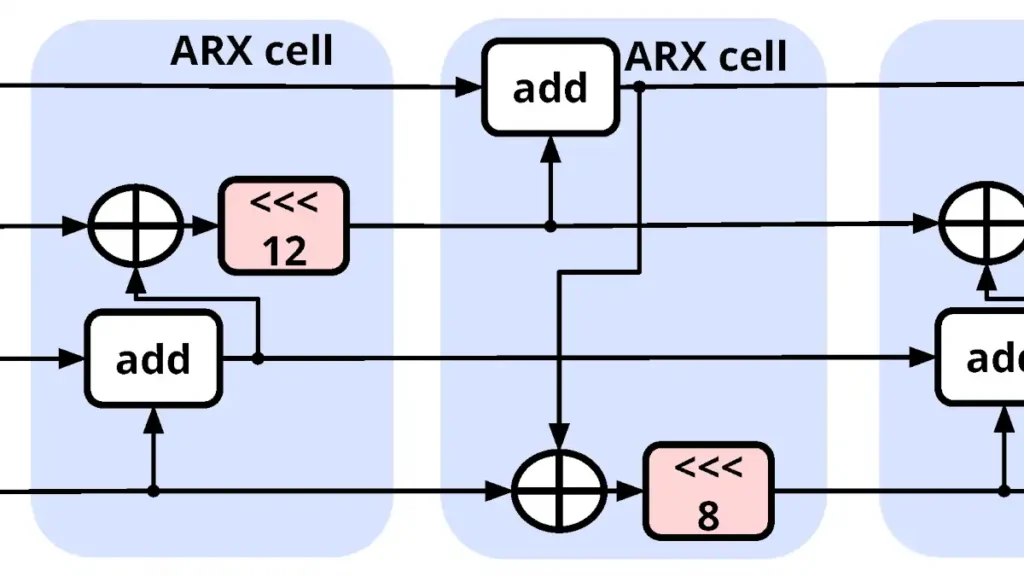
\includegraphics[width=0.9\textwidth]{figures/fig07-chacha20-1024x576.png}
\end{minipage}

